\documentclass[10pt,journal,compsoc]{IEEEtran}

\usepackage{verbatim}
\usepackage{url}
\usepackage{graphicx}

\usepackage{xspace}
\newcommand{\FC}       {Freechains\xspace}
\newcommand{\reps}     {\emph{reps}\xspace}
\newcommand{\onerep}   {\emph{1~rep}\xspace}
\newcommand{\nreps}[1] {\emph{#1~reps\xspace}}
\newcommand{\code}[1]  {\texttt{\footnotesize{#1}}}
\newcommand{\Xon} {$1{\rightarrow}N$\xspace}
\newcommand{\Xno} {$1{\leftarrow}N$\xspace}
\newcommand{\Xnn} {$N{\leftrightarrow}N$\xspace}
\newcommand{\Xoo} {$1{\leftrightarrow}1$\xspace}
\newcommand{\Xo}  {$1{\hookleftarrow}$\xspace}
\newcommand{\lin}[1]{(\emph{ln. #1}\xspace)}

\renewcommand{\theenumi}{\alph{enumi}}

\hyphenation{off-line}

\begin{document}

\title{
    Symmetric Peer-to-Peer Applications
}

\author{
    Francisco Sant'Anna~\IEEEmembership{Department of Computer Science, Rio de Janeiro State University}
}

\IEEEtitleabstractindextext{%
\begin{abstract}
In multi-node collaborative applications, such as shared online documents,
users can interact remotely and yet share the exact same experience as if they
were in a single machine.
%
In this work, we propose a middleware for \emph{symmetric peer-to-peer
applications} in which decentralized instances can broadcast asynchronous
events and yet conform to identical behavior.
%
Nodes are allowed to join and leave the network at any time.
Application developers must adhere to a restricted API, which is deterministic,
stateless, and only supports pre-allocated memory.
%
The middleware is responsible for synchronizing the events in a global shared
timeline across the network.
Based on memory snapshots and deterministic simulation, a ``time machine'' can
rollback conflicting peers to resynchronize their state.
%
TODO: application, results
\end{abstract}

\begin{IEEEkeywords}
collaboration, determinism, peer-to-peer, time machine
\end{IEEEkeywords}}

\maketitle

% TOTAL: 12 pages

\section{Introduction}
\label{sec.introduction}

\IEEEPARstart{C}{ollaborative} networked applications allow multiple users to
interact remotely and yet share the same experience in real time.
Examples of these \emph{symmetric distributed applications}~\cite{gals} are
shared documents, watch parties, and multi-player games.
%
In order to reproduce the exact behavior in multiple devices, the application
must be able to synchronize time and execution across the network.
In addition, since users can interact asynchronously with the application,
event occurrences must somehow be synchronized back across devices.

A common approach towards symmetric applications is to introduce a middleware
to orchestrate events and time in the network~\cite{gals,croquet}.
This way, applications developers can rely on middleware primitives to trigger
events, which are intercepted and synchronized in a global shared timeline
across the network.
Developers must also restrict themselves to deterministic and stateless calls
only, such that execution can be equally reproduced in all nodes according to
the shared timeline.
However, current solutions depend on a central server to interconnect network
nodes and determine the shared timeline.

In this work, we propose \emph{symmetric peer-to-peer applications}, which
do not rely on central servers for coordination.
Nodes in the application form a dynamic graph network and communicate only
with direct neighbours.
Events are flooded in the graph and are triggered locally with a small delay
to consider the network latency.
To deal with events received out of order or too late, a distributed time
machine can rollback peers to a previous state and reapply events in order and
in time.
Our main contribution is the design of a middleware that runs on each peer to
ensure that all peers
    (a) meet event deadlines,
    (b) advance in sync in real time, and
    (c) can leave and join the network and remain symmetric.

TODO: application, results

In Section~\ref{sec.related}, we revisit existing solutions for symmetric
distributed applications.
In Section~\ref{sec.tml}, we detail our proposed middleware.
In Section~\ref{sec.app}, ...
In Section~\ref{sec.eval}, ...
In Section~\ref{sec.conclusion}, ...

- assumptions
    - correct (non-malicious) nodes

- local first
- p2p
- less restrictive (compared to CRDTs)
- semantic events
    - limitation b/c of rollbacks
    - features b/c of network traffic

\section{Related Work}
\label{sec.related}

% docs.google.com/spreadsheets/d/1CpMmEgabJq2XQeTDW_BNCV4JWrcMlELuaEjDtw7kwg0/
\begin{figure}[t]
  \centering
  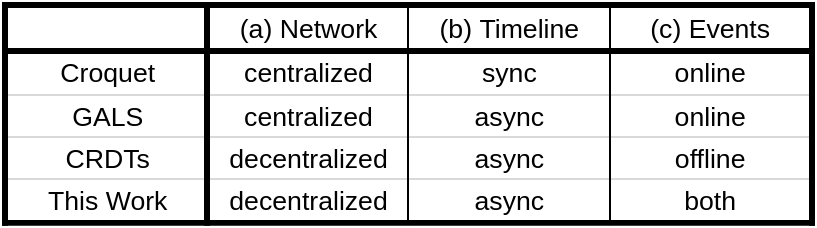
\includegraphics[width=\linewidth]{table}
  \caption{
    Related work regarding
        (a) how the network is organized,
        (b) how global time is determined, and
        (c) how events are propagated and applied.
    \label{fig.table}
  }
\end{figure}

\begin{figure*}[p]
  \centering
  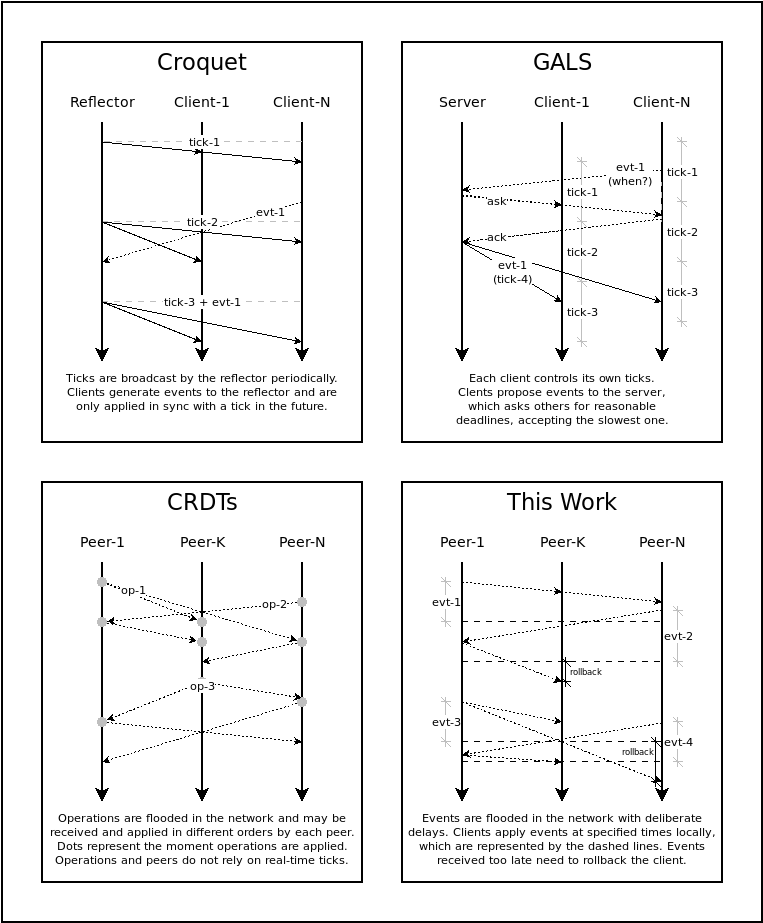
\includegraphics[width=\linewidth]{algos}
  \caption{
    \label{fig.algos}
    Four approaches to symmetric distributed applications: Croquet, GALS,
    CRDTs, and this work.
    The vertical arrows in parallel represent the timelines in nodes in the
    network.
    The arrows crossing nodes represent communication between them.
  }
\end{figure*}

In this section, we revisit existing solutions for symmetric distributed
applications.
We focus on
    (a) how the network is organized,
    (b) how global time is determined, and
    (c) how events are propagated and applied.
Figure~\ref{fig.table} compares selected works regarding these aspects.

Croquet%
\footnote{Croquet.io: https://croquet.io/}~\cite{croquet} guarantees
bit-identical real-time behavior for every user in a collaborative
distributed environment.
%
As detailed in Figure~\ref{fig.algos}, a centralized \emph{reflector} issues
periodic ticks, such that all nodes in the network advance together according
to a synchronized global shared clock.
If an user generates an event, it is delayed and sent back to the reflector,
which broadcasts the event in the next tick, which all nodes apply in sync
(including the originating node).
%
Croquet takes periodic snapshots of the whole application state in order to
support late joins to a running session.
The new node just needs to restore the latest snapshot and simulate the
remaining events to reach the current running state.
%
As indicated in Figure~\ref{fig.table}, Croquet relies on a centralized
network, in which nodes advance in sync, and in which event outcomes depend
on the central server to be online.

GALS~\cite{gals} shares the same goals with Croquet, but with some tradeoffs,
mostly favoring clients with slow connections.
As detailed in Figure~\ref{fig.algos}, instead of advancing ticks in sync with
the server, clients have their own local clocks.
Also, event generation is delayed dynamically according to the slowest client.
%
On the one hand, ticks do not generate any traffic and clients have smooth
frame transitions, even those with poor connections.
On the other hand, event generation requires two round trips to the server and
clients may experience occasional freezes.
The syncing protocol also requires bookkeeping to deal with clock drifts and
client disconnections~\cite{gals}.
%
As indicated in Figure~\ref{fig.table}, GALS relies on a centralized
network, in which nodes advance independently, and in which event outcomes
depend on the central server to be online.

In both solutions, the network advances together as a whole in real time, with
a total order among events, which is determined by a central server that must
be permanently online.
All clients compute the events in sequence, respecting their timestamps, and
using only deterministic and stateless calls.
This way, it is guaranteed that all clients reach the same state, also going
through bit-identical steps.

An antagonistic approach to deterministic reactions to events is to model the
application with conflict-free replicated data types (CRDTs)~\cite{crdts}.
CRDTs are designed in such a way that all operations are commutative, so that
the order in which they are applied does not affect the final outcome.
%
As detailed in Figure~\ref{fig.algos}, peers can communicate operations
directly to each other with no central authority.
Also, since operations need not to be ordered, they can be applied at the
very first moment they are generated or received, even if the peers are
offline.
%
Since operations must be commutative, it is not possible to timestamp them
in a global shared clock.
Hence, there is no notion of a timeline in which peers go through
bit-identical steps, but they do eventually reach the same state.
%
On the one hand, the main advantage of CRDTs is the support for local-first
software~\cite{local}, since they can work offline in the same way as online.
On the other hand, they provide very restrictive APIs (the CRDTs themselves),
and do not support real-time consensus among peers.
%
As indicated in Figure~\ref{fig.table}, CRDTs work on decentralized networks,
in which peers advance independently, and in which operations can be applied
immediately, even while offline.
%
Automerge along with its accompanying Hypermerge peer-to-peer infrastructure
is an example of an implementation of decentralized
CRDTs~\cite{p2p.automerge,p2p.pushpin}.

In this work, as indicated in Figure~\ref{fig.table}, our goal is to support
peer-to-peer real-time symmetric execution, while still tolerating offline and
out-of-order event generation.
%
As detailed in Figure~\ref{fig.algos}, peers have independent timelines and
can communicate events directly to each other.
Events are delayed to be able to reach other peers in time.
In the case a deadline is missed, the peer rolls back in time and then fast
forwards execution until it catches real-time behavior again.
%
Like Croquet and GALS, peers compute events in sequence using only
deterministic and stateless calls.

Regarding decentralized time machines, Fusion%
\footnote{Fusion: \url{https://doc.photonengine.com/en-us/fusion}}
is a state synchronization networking library for the Unity game engine.
It provides networked tick-based simulation in two modes: client-server
(\emph{hosted mode}) and peer-to-peer (\emph{shared mode}).
The hosted mode is based on continuous memory snapshots, which allows for
full rollbacks when clients diverge.
However, the shared mode is less powerful and only supports eventual
consistency among clients.
We presume that continuous memory snapshots would be too costly without a
central server.

Regarding single-user time machines, the video game Braid%
\footnote{\url{Braid: http://braid-game.com/}}
is designed on the assumption that players have unrestricted rollbacks as part
of the game mechanics.
Like Fusion, the implementation is based on continuous memory snapshots,
instead of deterministic simulation as we propose in this work.
%
Schuster~\cite{tml.js} proposes a simple API for time travelling in
event-driven JavaScript:
    \code{init()} to return an initial state;
    \code{handle(evt,mem)} to process events and modify state; and
    \code{render(mem)} to output the current state.
As we describe next, we use a similar approach by separating mutation from
rendering~\cite{tml.alive}.

\section{The Middleware \& Programming API}
\label{sec.tml}

In this section, we describe the architecture of our middleware and also the
API in which developers have to conform with.
%
The middleware is written in C and relies on the library \emph{SDL}%
\footnote{SDL: \url{www.libsdl.org}}
to deal with the network and input events, such as timers, mouse clicks and
key presses.
The full source code%
\footnote{TODO}
is under 500 lines of code.

\begin{figure}[t]
    \centering
    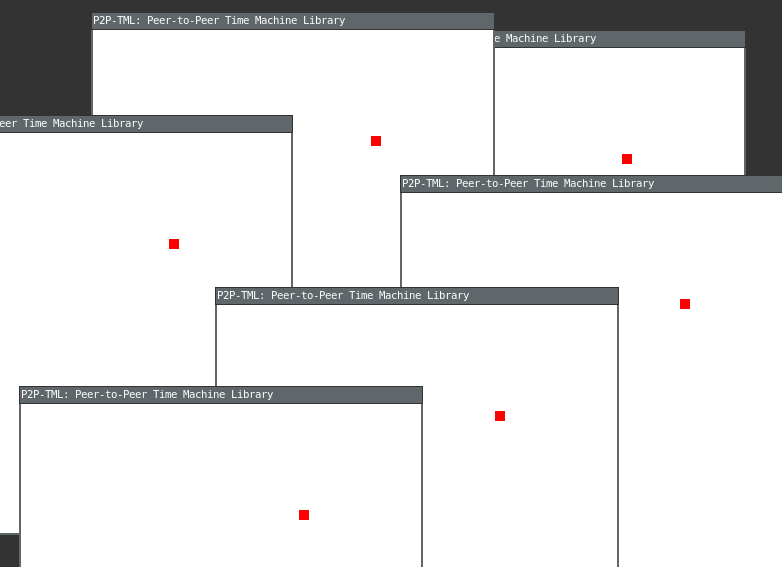
\includegraphics[width=\linewidth]{move}
    \caption[XXX] {
        A moving rectangle is controlled by peers connected indirectly.
        Users can press \code{↑ ↓ → ←} to change the direction of the
        rectangle or \code{SPACE} to pause the application.
        The inputs are applied simultaneously in all peers, as if they were
        mirrors of a single application.
        Video: \url{http://youtube.com/TODO}
        \label{fig.move}
    }
\end{figure}

We guide our discussion through the didactic example of Figure~\ref{fig.move},
in which multiple users use the arrow keys to control the direction of a
moving rectangle.
The six instances are connected in a peer-to-peer network, such that some
peers can only communicate indirectly.
%
The application is symmetric in the sense that if any peer presses a key, a
corresponding event is broadcast and applied in all peers simultaneously, as
if they were a single mirrored instance.
At any moment, if a peer pauses the application, all peers are guaranteed to
pause exactly at the same frame with the rectangle being ``bit-identically'' at
the same position.

\begin{figure}[t]
  \centering
  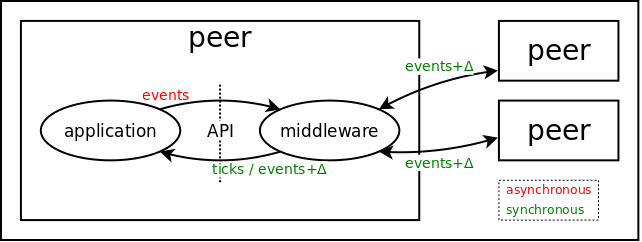
\includegraphics[width=\linewidth]{middleware}
  \caption{
    Applications generate asynchronous events and communicate through an API
    with the middleware.
    The middleware orchestrates the peers, synchronizing their ticks locally
    and broadcasting events with a delay.
    \label{fig.middleware}
  }
\end{figure}

In Figure~\ref{fig.middleware}, a peer is depicted as an application that uses
an API to communicate with the middleware.
The application itself is not aware of the network and has no direct access to
the other peers, which communicate transparently through the middleware.
The application generates asynchronous events that go through the middleware,
which synchronizes them with a timestamp in the future, such that all peers can
agree.
The middleware controls the execution of the application by issuing ticks and
synchronized events.

The main job of the middleware is to deal with the uncertainties of the
network in order to preserve the symmetric behavior across peers.
As described in the Introduction, the middleware ensures that all peers
    (a) meet event deadlines,
    (b) advance in sync in real time, and
    (c) can leave and join the network and remain symmetric:
%
\begin{enumerate}
\item \textbf{Event Deadlines:}
Due to the inherent latency of networks, peers generate events with a
deliberate delay so that they reach other peers in time to be applied in sync
in a common deadline.
%We first assume a predetermined delay for the sake of simplicity.
However, a peer that is locally ahead of time may receive an event that should
have been applied in the past, event considering the delay.
In this case, the middleware automatically rolls back the peer, applies the
event at the correct time, and then fast forwards the peer, re-applying all
remaining events up to the real time.
As we detail further, rolling back a peer requires to simulate its whole
execution from the beginning (or from a snapshot in between).
%
\item \textbf{Time Synchronization:}
Since peers run in different machines, their timelines will inevitably be out
of sync because:
    (a) applications are launched locally at different times, and
    (b) internal clocks may diverge over time.
The middleware assumes the maximum time among all peers the be the
``correct real time'', so that other peers must fast forward to catch up with
it.
Therefore, in order to determine the maximum time and synchronize the clocks,
the middleware proceeds as follows:
    (a) peers broadcast \code{SYNC} events periodically with their local
        times, and
    (b) if a peer is behind a received \code{SYNC}, it advances its frames
        proportionally faster to catch up in time.
%
\item \textbf{Peer Churn:}
Considering that we target peer-to-peer networks, it is important that the
middleware can handle arrival and departure of peers seamlessly.
When a peer leaves the network, nothing needs to be done.
The middleware just needs to ensure that a peer that joins the network receives
all events in order, which is trivial since they all hold an absolute
timestamp.
\end{enumerate}

\subsection{The Programming API}
\label{sec.tml.api}

The middleware expects to take full control of the application execution in
order to control its timeline and disseminate events in the network.
For this reason, the basic programming API is to call a \code{loop} function
passing a set of callbacks, which the middleware uses to communicate with the
application:

{\footnotesize
\begin{verbatim}
int main (void) {
    p2p_loop (
        1,              // peer identifier
        50,             // simulation FPS
        sizeof(G), &G,  // pre-allocated full state
        cb_ini,         // init/quit callback
        cb_sim,         // simulation callback
        cb_ren,         // rendering callback
        cb_evt          // events callback
    );
}
\end{verbatim}
}

The middleware assumes that each peer assigns to itself a unique identifier in
a contiguous range.
The FPS must be the same in all peers to ensure that the simulation executes
exactly the same.

\subsubsection{Application State}
\label{sec.tml.api.state}

The global variable \code{G} must hold the full application state.
This allows the middleware to take memory snapshots and rollback to a previous
state.
If dynamic allocation is required, it is necessary to hold a finite memory
pool in \code{G} with a custom allocator.
For instance, the moving rectangle application only requires to hold the
current position and direction:

{\footnotesize
\begin{verbatim}
struct {
    int x,  y;   // position
    int dx, dy;  // direction speed
} G;
\end{verbatim}
}

\subsubsection{Application Events}
\label{sec.tml.api.events}

The application generates events that need to be broadcast to the network so
that all peers behave the same.
In this sense, application events may differ from low-level local system
events, which may or may not be mapped 1-to-1 in the callback \code{cb\_evt}.

There middleware predefines two events for all applications:
    \code{P2P\_EVT\_START} represents the beginning of the simulation, and
    \code{P2P\_EVT\_TICK} called at every frame.
The application-specific events must be declared by the programmer in an
enumeration.
In our application, we define a new event \code{P2P\_EVT\_KEY} to represent key
presses:

{\footnotesize
\begin{verbatim}
enum {
    P2P_EVT_KEY = P2P_EVT_NEXT
};
\end{verbatim}
}

\subsubsection{Initialization Callback}
\label{sec.tml.api.cb_ini}

The middleware calls \code{cb\_ini} twice: at the beginning and at the end of
the loop.
It should be used to initialize (and finalize) the network topology, as well
as static globals that can live outside the simulation memory, such as the
window and image textures:

{\footnotesize
\begin{verbatim}
void cb_ini (int ini) {
    if (ini) {
        <...> // create the SDL window
        <...> // open the arrow PNG images
        // create peer links (peer-id, ip, port)
        p2p_link(2, "192.168.1.2", 5000);
    } else {
        <...> // destroy the SDL window
        <...> // destroy the arrow PNG images
        // destroy peer links
        p2p_unlink(2);
    }
}
\end{verbatim}
}

\subsubsection{Simulation Callback}
\label{sec.tml.api.cb_sim}

The middleware calls \code{cb\_sim} on every frame, passing an application
event, to affect the simulation state \code{G} deterministically.
The callback must never perform any side effects, such as stateful calls or
rendering frames.
In our example, we modify the state of the rectangle as follows:
    (a) reset its position and speed on \code{START},
    (b) increment its position based on the current speed on \code{TICK}, and
    (c) modify its speed based on \code{KEY}:

{\footnotesize
\begin{verbatim}
void cb_sim (p2p_evt evt) {
    switch (evt.id) {
        case P2P_EVT_START: // resets pos and speed
            G.x = G.y = G.dx = G.dy = 0;
            break;
        case P2P_EVT_TICK:  // increases position
            G.x += G.dx * VEL;
            G.y += G.dy * VEL;
            break;
        case P2P_EVT_KEY:  // modifies speed
            switch (evt.pay.i1) {
                case SDLK_UP:
                    G.dx = 0;
                    G.dy = -1;
                    break;
                <...> // same for other keys
            }
            break;
    }
}
\end{verbatim}
}

The calls to \code{cb\_sim} normally happen during real-time simulation, i.e.,
while the user is interacting with the application.
However, if the peer is out of sync, the middleware may ``time travel'' and
call the simulation many times to go back and forth and catch up with real
time.
This is the reason why we define \code{START} as an event like any other, since
travelling requires to simulate the execution from the beginning, event by
event.

\subsubsection{Rendering Callback}
\label{sec.tml.api.cb_ren}

Time travelling is also the reason why \code{cb\_sim} must be split from the
rendering callback \code{cb\_ren}~\cite{tml.js}, which would otherwise render
the screen multiple times while travelling.
%, which the middleware calls only on real-time frames.
In our example, \code{cb\_ren} just needs to redraw the rectangle at the
current position:

{\footnotesize
\begin{verbatim}
void cb_eff (void) {
    <...> // clears the SDL window
    // redraws the rectangle at the current position
    SDL_Rect r = { G.x, G.y, 20, 20 };
    SDL_DrawRect(&r);
}
\end{verbatim}
}

\subsubsection{Events Callback}
\label{sec.tml.api.cb_evt}

The \code{cb\_evt} callback is called by the middleware in real time, whenever
a local SDL event occurs.
This callback has two goals:
    (a) map and broadcast application events, and
    (b) provide instant feedback to the user.
As mentioned previously, not all local low-level events may generate
application events to be broadcast in the network.
The callback is allowed to perform side effects, such as modifying the network
topology, or exhibiting some feedback on the screen.
In our example, we only generate application events for the 5 key events, and
we also exhibit the pressed key in real time:

{\footnotesize
\begin{verbatim}
int cb_evt (SDL_Event* sdl, p2p_evt* evt) {
    if (sdl->type == SDL_KEYDOWN) {
        if (sdl->key == <any-of-the-keys>) {
            SDL_DrawImage(<img-of-the-key>);
            *evt = (p2p_evt){ P2P_EVT_KEY,sdl->key };
            return 1; // generate application event
        }
    }
    return 0; // otherwise, do not generate any event
}
\end{verbatim}
}

\subsection{Middleware Orchestration}
\label{sec.tml.middleware}

We now detail how the middleware orchestrates an application and ensures that
all peers
    (a) meet event deadlines,
    (b) advance in sync in real time, and
    (c) can leave and join the network and remain symmetric.

\subsubsection{Events Broadcasting}
\label{sec.tml.middleware.events}

As illustrated in Figure~\ref{fig.middleware}, events are broadcast between
peers with a timestamp in the future such that all peers are able to apply them
in sync.
%
To prevent broadcast cycles, event are tagged with a source peer and sequence
number.
Each peer keeps a vector with the highest sequence number it received from each
other peer, such that lower numbers can be ignored when received.
Higher numbers update the vector and trigger a broadcast to neighbours.
Since we rely on TCP connections, it is not possible to receive out-of-order
sequence numbers from the same source peer.
%
As mentioned in Section~\ref{sec.tml.api}, we assume that peers assign
themselves unique identifiers in a contiguous range.
The reasons are
    (a) to fit a \code{uint8\_t} size, and
    (b) to use a contiguous vector of sequence numbers.
Therefore, this is not a serious limitation, and a separate mechanism could be
used for assignment, with few modifications to core of the middleware.

When receiving an unseen event, the middleware also enqueues it in timestamp
order and calls the application callback \code{cb\_sim} at the appropriate
time.
The peers must keep the full queue in memory for two reasons:
    (a) receiving a late event may reorder the queue and require a time
        travel, and
    (b) peers that join the network need to receive all events.
%
Therefore, the middleware keeps a queue of ``packets'', which includes the
event and other metadata:

{\footnotesize
\begin{verbatim}
typedef struct {
    uint8_t  src;       // source peer
    uint32_t seq;       // sequence number
    uint32_t tick;      // tick to apply
    p2p_evt  evt;       // event id + payload
} p2p_pak;

struct {
    int i;              // next event to apply
    int n;              // number of events
    p2p_pak buf[MAX];   // queue of packets
} PAKS;
\end{verbatim}
}

\subsubsection{The Main Loop}
\label{sec.tml.middleware.loop}

The middleware main loop \code{p2p\_loop} is responsible for calling the
application callbacks, and also controlling its timeline.
The loop continuously checks for network packets, local inputs, and time ticks,
as follows:

{\footnotesize
\begin{verbatim}
01  void p2p_loop (...,cb_ini,cb_sim,cb_ren,cb_evt) {
02    cb_ini(1);
03    cb_sim(<P2P_EVT_START>);
04
05    while (<app-running>) {
06      if (<next-packet>) {
07        // fast forward if I'm late
08        if (<packet-sync-future>) {
09          p2p_travel(<now>, <packet-sync-time>);
10        }
11
12        // travel back & forth if I'm early
13        if (<packet-evt-past>) {
14          p2p_travel(<now>, <packet-evt-time>);
15          p2p_travel(<packet-evt-time>, <now>);
16        }
17
18        // simulate in real time if I'm on time
19        if (<packet-evt-ok>) {
20          cb_sim(<packet-evt>);
21          cb_ren();
22        }
23      }
24
25      if (<next-input>) {
26        // broadcast event from local
27        p2p_evt evt;
28        if (cb_evt(&evt)) {
29          p2p_bcast(<future>, &evt);
30        }
31      }
32
33      // simulate tick in real time
34      if (<next-tick>) {
35        cb_sim(<P2P_EVT_TICK>);
36        <application-snapshot-every-second>
37        cb_ren();
38      }
39    }
40
41    cb_ini(0);
42  }
\end{verbatim}
}

The function receives the application callbacks as arguments \lin{1}
(Section~\ref{sec.tml.api}).
We first (and last) call \code{cb\_ini} \lin{2,41} to initialize (and finalize)
the application.
Then, we call \code{cb\_sim} \lin{3}, passing the event \code{START} to start
the application in real time
(Sections~\ref{sec.tml.api.events}~and~\ref{sec.tml.api.cb_sim}).
The main loop \lin{5--39} checks continuously for network packets \lin{6--23},
local input events \lin{25--31}, and time ticks \lin{33--38}.

Regarding network packets, if we receive a time synchronization packet
\code{SYNC} from the future \lin{7--10}, then the we fast forward the
application to catch up in time (Section~\ref{sec.tml}.b).
If we receive an event that should have been applied in the past \lin{12--16},
then we travel back and forth (Section~\ref{sec.tml}.a).
Otherwise, we just apply the event in real time \lin{18--22}
(Section~\ref{sec.tml.api.cb_sim}).
We detail the function \code{p2p\_travel} in
Section~\ref{sec.tml.middleware.travel}.
%
Regarding local inputs, we call \code{cb\_evt} \lin{26--30} to signal if the
event should be broadcast, also transforming it to an application event
(Section~\ref{sec.tml.api.cb_evt}).
%
Regarding time tick, we call \code{cb\_sim} and \code{cb\_ren} in real time
\lin{33--38}.
The middleware also takes periodic snapshots of the application state to
rollback and assist time travelling (Section~\ref{sec.tml.api.state}).

\subsubsection{The Time Machine}
\label{sec.tml.middleware.travel}

The last important mechanism of the middleware is the time machine, which
allows to move the application back and forth in time:

{\footnotesize
\begin{verbatim}
01  void p2p_travel (int from, int to) {
02    for (i=from..to) {
03      int bef = <tick-of-snapshot-before-i>
04      <restore-snapshot-at-bef>
05      for (j=bef..i) {
06        cb_sim(<tick-or-evt-at-j>)
07      }
08      cb_ren();
09      <delay-ms>
10    }
11  }
\end{verbatim}
}

The function \code{p2p\_travel} time travels, starting at tick \code{from},
tick by tick, until it reaches tick \code{to} \lin{2--10}.
The loop can go in any direction in time, i.e., \code{from} may be higher than
\code{to}.
At each step, we need to find the tick \code{bef} with the closest past
snapshot \lin{3}, restore it \lin{4}, and than simulate the remaining steps
from the snapshot to the desired tick \lin{5--7}.
We also exhibit each step with a small delay \lin{8--9} so that users
experience smooth time transitions.

\subsubsection{Summary}
\label{sec.tml.middleware.summary}

This section provided an overview of the middleware implementation to answer,
in concrete terms, how it ensures the desired properties enumerated in the
Introduction and at the beginning of Section~\ref{sec.tml.middleware}:
    (a) peers meet event deadlines either in real time \lin{18--21} or
        travelling back and forth in time \lin{12--16}
        (Section~\ref{sec.tml.middleware.loop});
    (b) peers synchronize their clocks with periodic \code{SYNC} packets that
        fast forwards late peers \lin{7--10}
        (Section~\ref{sec.tml.middleware.loop}); and
    (c) peers can join the network at any time and still catch up in time by
        receiving the full event history
        (Section~\ref{sec.tml.middleware.events}).

\section{Evaluation}
\label{sec.eval}

In this section, we evaluate if (and to what extent) our design meets its goals
to ensure that all peers (a) meet event deadlines, (b) advance in sync in real
time, and (c) can leave and join the network and remain symmetric.
%
We simulate an application varying the network topology, latency, and churn, as
well as the frequency and deadlines of events.
%
We then measure (a) the recurrence of time travels, (b) the real-time pace of
peers, and (c) the correctness of unstable peers, such that they validate our
goals above, respectively.

Regarding (a), if a peer experiences a time travel, it means that it received
an event after its deadline.
We count all time travel occurrences during the simulation.
%
Regarding (b), we use an absolute simulation clock to track, in real time, the
execution pace of each peer in comparison to a reference peer most advanced in
time.
%
Regarding (c), we designate some peers to leave and join the network
periodically to assert that they catch up with the other peers in real time.

\begin{figure*}[t]
  \centering
  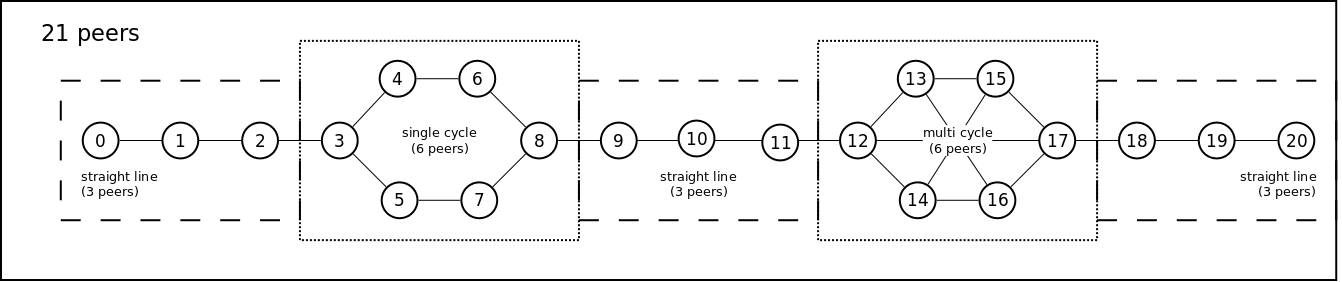
\includegraphics[width=\linewidth]{topo}
  \caption{
    \label{fig.topo}
    TODO
  }
\end{figure*}

We simulate the application with $21$ peers using the mixed topology of
Figure~\ref{fig.topo}, with peers organized in straight lines, long cycles, and
short cycles.
%
In order to have an absolute clock to compare peers, we use a single machine
to simulate all peers, and merge their logs into a single file constituting a
shared timeline.
%
We simulate the network latency and clock drift in software with random delays.

We now detail how we instrument the middleware implementation measure the
properties above:
%
\begin{enumerate}
%
\item \textbf{Recurrence of time travels:}
Every time a peer is ahead of time and needs to travel back, we output its id
and how much ticks it needs to travel back.
At the end, we measure the percentage of the sum of all time travel ticks over
the total simulation ticks.
As an example, if all peers sum $1000$ time travel ticks over $100k$
accumulated simulation ticks, then the final measure is $1\%$.
%
\item \textbf{Real-time pace of peers:}
We start each peer with a random delay of up to $10s$ to force a time mismatch.
We also force exaggerated clock drifts in random peers ($1ms$ every $1h$).
and then verify if they synchronize and remain synchronized during the whole
simulation.
We teak the middleware to output its current tick every $100ms$.

More concretely, we measure the percentage o ticks diverging from the reference
peer (e.g., $1\%$, if .

%
\end{enumerate}

For instance, if the reference peer signals $T$ and then a peer signals $T-dt$,
than we.
That would be the case when a source peer generates an event with a small
deadline in comparison to the latency to the farthest destination peer.

We run the simulation for 5 minutes and, since we start the measures after 1 minute

- VARIABLES
- number of nodes
- topology
    - distance b/w nodes
    - number of edges
- latency b/w nodes
- freq of events
- ~FPS~
- future delta

- RESULTS
- time travels
- ~real time~
- ~enter leave~ (catches up?)

-- use of space for snapshots
-    - limit to go back?
-    - super nodes? (when connecting, pass tick, may close if tick<last)

-- start with random deltas
\section{TODO}

TODO: simpler than vector clocks, absolute times are correct

- p2p links por fora, como um servico TCP local

We make some assumptions about the network, which are assigned externally to
the middleware:
%
\begin{itemize}
\item Peers identifiers are assigned externally to the middleware.
\item Topology is dynamic, but also assigned externally

\end{itemize}
%
Except for the last item, we claim that the others can be solved externally,
without affecting the middleware.
For instance,
- orthogonal and would not affect the other algorithms in the middleware

, which we claim that could be
solved further:
- ids are outside
- topology, dynamic but outside
- fixed maximum nodes
- fixed latency
We claim that Use external protocols
For instance, latency is only a constant, no problem being a variable

- non-malicious nodes

\section{Application}
\label{sec.app}

\section{Conclusion}
\label{sec.conclusion}

\bibliographystyle{IEEEtran}
\bibliography{tpd-22}

\begin{comment}
\begin{IEEEbiography}[{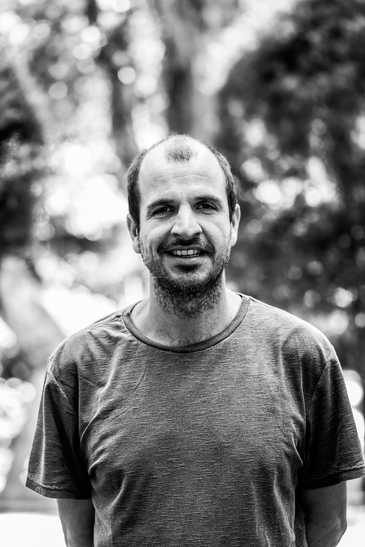
\includegraphics[width=1in,height=1.25in,clip,keepaspectratio]{chico}}]{Francisco Sant'Anna}
received his PhD degree in Computer Science from PUC-Rio, Brazil in
2013.
In 2016, he joined the Faculty of Computer Science at the Rio de Janeiro State
University, Brazil.
His research interests include Programming Languages and Concurrent \&
Distributed Systems.
\end{IEEEbiography}
\end{comment}

\end{document}
